\documentclass[10pt,aspectratio=169]{beamer}

\usetheme{Madrid}
\usecolortheme{default}

\usepackage[spanish, es-tabla]{babel}
\usepackage[utf8]{inputenc}
\usepackage[T1]{fontenc}
\usepackage{graphicx}
\usepackage{booktabs}
\usepackage{tikz}
\usetikzlibrary{arrows.meta, positioning, calc}

\definecolor{urjcred}{RGB}{164, 0, 39}
\definecolor{softblue}{RGB}{43, 116, 181}
\definecolor{softgreen}{RGB}{65, 150, 95}
\definecolor{softorange}{RGB}{214, 124, 47}

\setbeamercolor{structure}{fg=urjcred}
\setbeamercolor{title}{fg=white,bg=urjcred}
\setbeamercolor{frametitle}{fg=white,bg=urjcred}
\setbeamercolor{section in head/foot}{fg=white,bg=urjcred}
\setbeamertemplate{navigation symbols}{}
\makeatletter
\setbeamertemplate{footline}{%
    \leavevmode%
    \hbox{%
        \begin{beamercolorbox}[wd=.78\paperwidth,ht=2.4ex,dp=1ex,leftskip=0.35cm]{section in head/foot}%
            \usebeamerfont{section in head/foot}\insertsection
        \end{beamercolorbox}%
        \begin{beamercolorbox}[wd=.22\paperwidth,ht=2.4ex,dp=1ex,rightskip=0.35cm plus1fil]{section in head/foot}%
            \usebeamerfont{section in head/foot}\hfill\insertframenumber/\inserttotalframenumber
        \end{beamercolorbox}%
    }%
}
\makeatother

\title[IA explicativa y EEG]{IA explicativa aplicada a la detección de emociones a través de señales EEG}
\author[Liam Saborido Sueiro]{Liam Saborido Sueiro}
\institute[URJC]{Grado en Ingeniería de Robótica Software\\Escuela de Ingeniería de Fuenlabrada}
\date{Curso académico 2025--2026}

\AtBeginSection[]{
    \begin{frame}[plain]
        \begin{tikzpicture}[remember picture,overlay]
            \node[align=center, text=urjcred, font=\Huge\bfseries, text width=11.5cm]
                at (current page.center)
                {\insertsection};

            \draw[urjcred, line width=1.1pt]
                ([xshift=-2.1cm,yshift=-0.72cm]current page.center)
                -- ([xshift=2.1cm,yshift=-0.72cm]current page.center);
        \end{tikzpicture}
    \end{frame}
}

\begin{document}

\begin{frame}[plain]
    \begin{tikzpicture}[remember picture,overlay]
        \fill[urjcred] ([xshift=1.25cm,yshift=-2.0cm]current page.north west)
            rectangle ([xshift=-1.25cm,yshift=-4.2cm]current page.north east);

        \node[align=center, text=white, font=\Large\bfseries, text width=11.5cm]
            at ([yshift=-3.1cm]current page.north)
            {IA explicativa aplicada a la detección\\[1mm]
            de emociones a través de señales EEG};

        \node[anchor=south west] at ([xshift=0.75cm,yshift=0.45cm]current page.south west)
            {
\includegraphics[width=0.16\textwidth]{../memoria/figs/logo_urjc.jpg}};

        \node[anchor=south east, align=right, font=\small] at ([xshift=-0.75cm,yshift=0.62cm]current page.south east)
            {Curso académico 2025--2026};
    \end{tikzpicture}

    \vspace{4.55cm}
    \begin{center}
        {\small Trabajo Fin de Grado}

        \vspace{0.18cm}
        {\small Escuela de Ingeniería de Fuenlabrada}\\
        {\small Grado en Ingeniería de Robótica Software}

        \vspace{0.45cm}
        {\normalsize Liam Saborido Sueiro}

        \vspace{0.25cm}
        {\small Tutor: Álvaro García López}\\
        {\small Co-tutor: Julio Salvador Lora Millán}
    \end{center}
\end{frame}

\begin{frame}[plain]
    \begin{tikzpicture}[remember picture,overlay]
        \node[anchor=south east, align=right] at ([xshift=-0.65cm,yshift=0.55cm]current page.south east) {
            
\includegraphics[width=0.10\textwidth]{../memoria/figs/by-sa.png}\\[1.5mm]
            {\scriptsize Creative Commons}\\[-0.5mm]
            {\scriptsize Attribution-ShareAlike 4.0 International}
        };
    \end{tikzpicture}
\end{frame}

\begin{frame}{Índice}
    \centering
    \vspace{0.05cm}
    \begin{tikzpicture}[
        numero/.style={
            circle,
            minimum size=0.62cm,
            fill=urjcred,
            text=white,
            font=\large\bfseries
        }
    ]
        \foreach \texto [count=\n] in {
            Introducción,
            Objetivos,
            Desarrollo del sistema,
            Resultados,
            Conclusiones
        } {
            \node[numero] at (-3.55,{1.65-0.86*(\n-1)}) {\n};
            \node[anchor=west, font=\LARGE\bfseries, text=black!88]
                at (-3.0,{1.65-0.86*(\n-1)}) {\texto};
        }
    \end{tikzpicture}
\end{frame}

\section{Introducción}

\begin{frame}{¿Qué es el EEG?}
    \vspace{0.05cm}
    \begin{columns}[c,onlytextwidth]
        \begin{column}{0.50\textwidth}
            \begin{tikzpicture}[
                idea/.style={
                    rectangle,
                    rounded corners=3pt,
                    fill=urjcred!8,
                    draw=urjcred!35,
                    text width=5.0cm,
                    minimum height=1.02cm,
                    align=left,
                    font=\small,
                    inner xsep=9pt
                }
            ]
                \node[idea] (a) {\textbf{EEG}\\Actividad eléctrica cerebral};
                \node[idea, below=0.36cm of a] (b) {\textbf{Electrodos}\\Colocados sobre el cuero cabelludo};
                \node[idea, below=0.36cm of b] (c) {\textbf{Canales}\\Una señal por cada posición};
            \end{tikzpicture}
        \end{column}

        \begin{column}{0.47\textwidth}
            \centering
            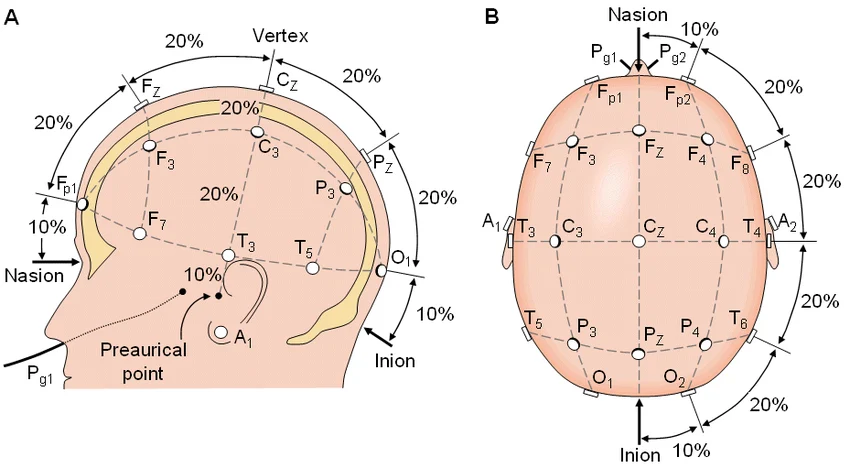
\includegraphics[width=0.86\textwidth]{../memoria/figs/sistema_10_20.png}

            \vspace{0.1cm}
            {\scriptsize Sistema internacional 10--20}
        \end{column}
    \end{columns}
\end{frame}

\begin{frame}{Señal por canales}
    \centering
    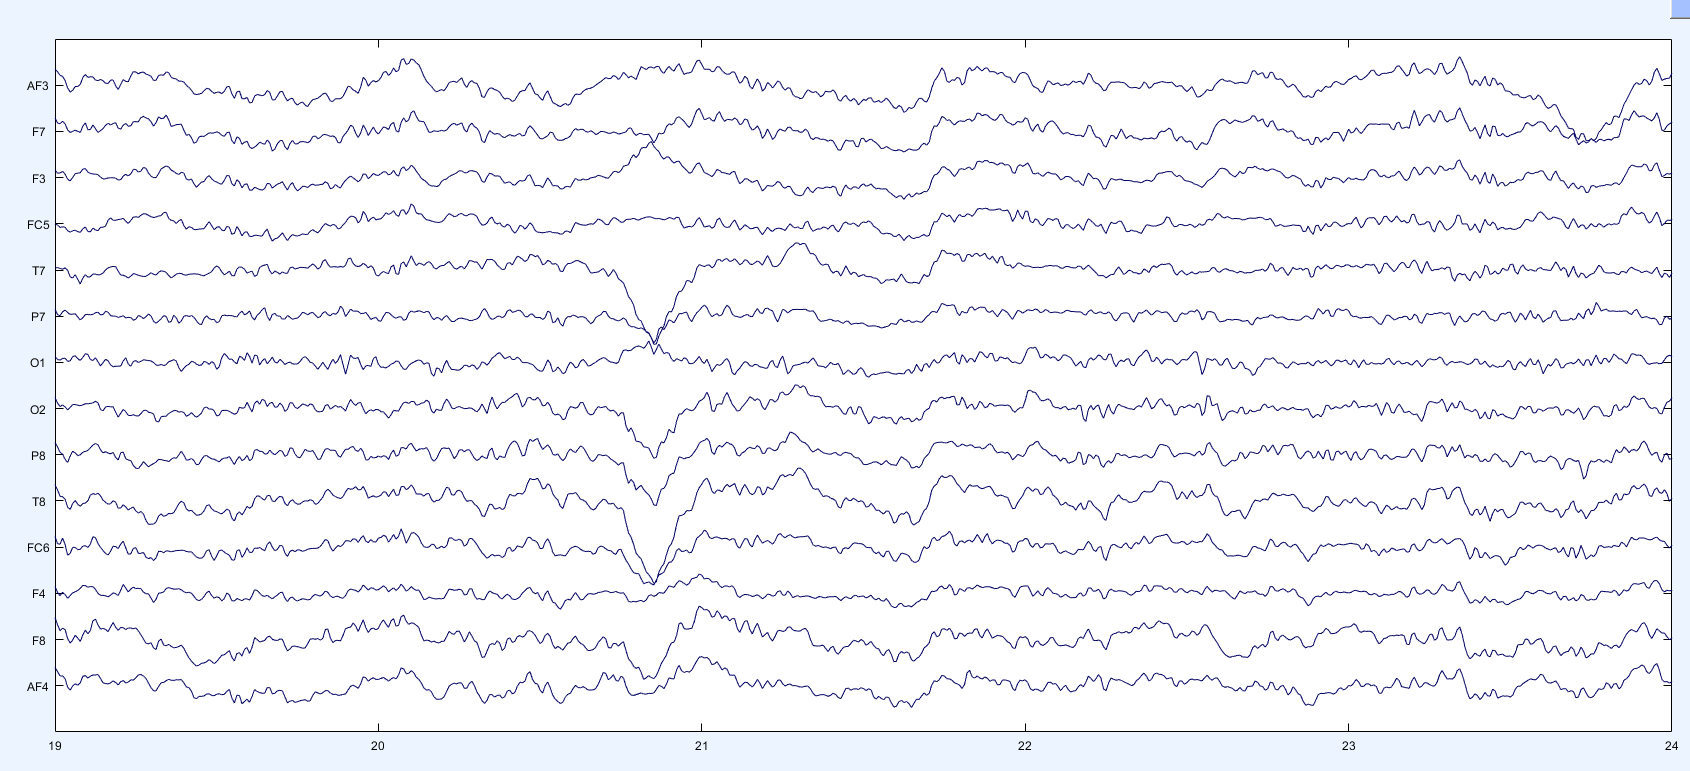
\includegraphics[width=0.82\textwidth]{figs/channels.png}

    \vspace{0.25cm}
    \begin{center}
        {\small Cada canal registra una señal temporal distinta, asociada a una posición del montaje.}
    \end{center}
\end{frame}

\begin{frame}{Motivación}
    \begin{columns}[c,onlytextwidth]
        \begin{column}{0.38\textwidth}
            \begin{tikzpicture}[
                motivo/.style={
                    rectangle,
                    rounded corners=3pt,
                    fill=urjcred!8,
                    draw=urjcred!35,
                    text width=4.0cm,
                    minimum height=1.0cm,
                    align=left,
                    font=\small,
                    inner xsep=8pt
                }
            ]
                \node[motivo] (a) {\textbf{Prueba del sueño}\\Primer contacto con señales EEG};
                \node[motivo, below=0.4cm of a] (b) {\textbf{Pregunta}\\¿Puede un modelo de IA entender estas señales?};
            \end{tikzpicture}
        \end{column}

        \begin{column}{0.58\textwidth}
            \centering
            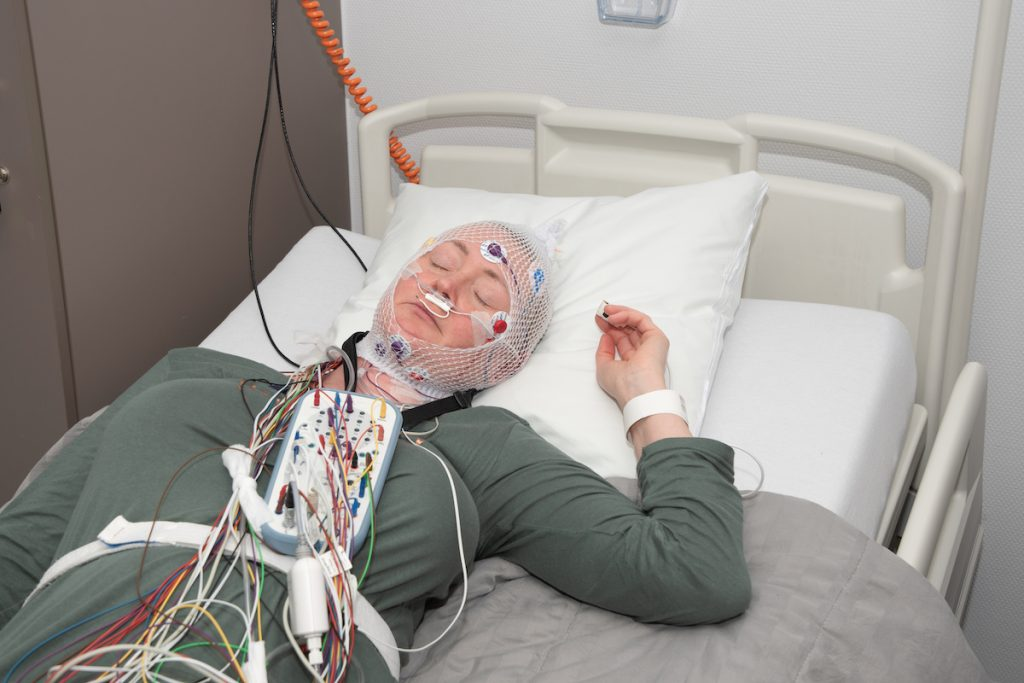
\includegraphics[width=0.92\textwidth]{figs/prueba_sueno.png}
        \end{column}
    \end{columns}
\end{frame}

\begin{frame}{Más allá de lo observable}
    \centering
    \begin{tikzpicture}[
        header/.style={
            rectangle,
            rounded corners=5pt,
            fill=urjcred!8,
            draw=urjcred!38,
            text width=10.2cm,
            minimum height=0.72cm,
            align=center,
            font=\small\bfseries
        },
        pista/.style={
            rectangle,
            rounded corners=5pt,
            fill=black!5,
            draw=black!24,
            text width=3.15cm,
            minimum height=0.78cm,
            align=center,
            font=\small
        },
        caso/.style={
            rectangle,
            rounded corners=5pt,
            fill=softblue!9,
            draw=softblue!38,
            text width=3.15cm,
            minimum height=0.82cm,
            align=center,
            font=\scriptsize
        },
        cierre/.style={
            rectangle,
            rounded corners=6pt,
            fill=softgreen!13,
            draw=softgreen!45,
            text width=7.1cm,
            minimum height=0.86cm,
            align=center,
            font=\small\bfseries
        }
    ]
        \node[header] at (0,2.35) {¿Cómo reconocemos normalmente una emoción?};
        \node[pista] at (-3.85,1.38) {Voz y palabras};
        \node[pista] at (0,1.38) {Gestos};
        \node[pista] at (3.85,1.38) {Expresión facial};

        \node[header] at (0,0.18) {Hay situaciones en las que eso no basta};
        \node[caso] at (-3.85,-0.82) {dificultades\\de comunicación};
        \node[caso] at (0,-0.82) {expresión\\reducida};
        \node[caso] at (3.85,-0.82) {contexto\\médico};

        \draw[-{Latex[length=2.2mm]}, thick, draw=black!45] (0,-1.38) -- (0,-1.78);
        \node[cierre] at (0,-2.28) {Señales EEG para reconocer emociones};
    \end{tikzpicture}
\end{frame}

\begin{frame}{¿Por qué IA explicable?}
    \begin{columns}[c,onlytextwidth]
        \begin{column}{0.64\textwidth}
            \begin{beamercolorbox}[rounded=true,sep=0.18cm,wd=\textwidth,center]{block body}
                {\small\bfseries Modelo explicable}

                \vspace{0.15cm}
                \begin{columns}[c,onlytextwidth]
                    \begin{column}{0.28\textwidth}
                        \centering
                        
\includegraphics[height=1.95cm]{figs/akinator.png}
                    \end{column}
                    \begin{column}{0.68\textwidth}
                        \centering
                        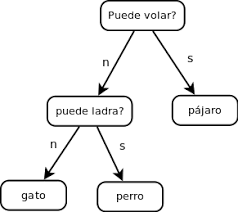
\includegraphics[width=\textwidth]{../memoria/figs/Arbol_decision.png}
                    \end{column}
                \end{columns}

                \vspace{0.18cm}
                \begin{tikzpicture}
                    \node[
                        rectangle,
                        rounded corners=3pt,
                        fill=softgreen!12,
                        draw=softgreen!45,
                        text width=6.4cm,
                        align=center,
                        minimum height=0.62cm,
                        font=\scriptsize
                    ] {Preguntas sucesivas hasta llegar a una decisión};
                \end{tikzpicture}
            \end{beamercolorbox}
        \end{column}

        \begin{column}{0.33\textwidth}
            \begin{beamercolorbox}[rounded=true,sep=0.18cm,wd=\textwidth,center]{block body}
                {\small\bfseries Caja negra}

                \vspace{0.22cm}
                
\includegraphics[height=1.75cm]{figs/chatgpt.png}

                \vspace{0.35cm}
                \begin{tikzpicture}
                    \node[
                        rectangle,
                        rounded corners=3pt,
                        fill=black!6,
                        draw=black!30,
                        text width=3.45cm,
                        align=center,
                        minimum height=0.95cm,
                        font=\scriptsize
                    ] {Predice, pero no siempre\\muestra cómo llega\\a la respuesta};
                \end{tikzpicture}
            \end{beamercolorbox}
        \end{column}
    \end{columns}

    \vspace{0.38cm}
    {\small En aplicaciones médicas, acertar no es suficiente: también hay que justificar la decisión.}
\end{frame}

\begin{frame}{Emociones analizadas}
    \centering
    \vspace{0.15cm}
    \begin{tikzpicture}[
        emocion/.style={
            rectangle,
            rounded corners=5pt,
            minimum width=3.35cm,
            minimum height=2.1cm,
            align=center,
            font=\small,
            draw=black!25,
            line width=0.5pt
        }
    ]
        \node[emocion, fill=red!16, draw=red!35] (joy) {
            {\Large\bfseries JOY}\\[2mm]
            respuesta positiva
        };
        \node[emocion, fill=green!16, draw=green!35!black, right=0.55cm of joy] (neutro) {
            {\Large\bfseries NEUTRO}\\[2mm]
            estado de referencia
        };
        \node[emocion, fill=blue!14, draw=blue!35, right=0.55cm of neutro] (sad) {
            {\Large\bfseries SAD}\\[2mm]
            respuesta negativa
        };
    \end{tikzpicture}

    \vspace{0.55cm}
    \begin{tikzpicture}
        \node[
            rectangle,
            rounded corners=3pt,
            fill=urjcred!8,
            draw=urjcred!35,
            text width=9.4cm,
            align=center,
            minimum height=0.9cm,
            font=\small
        ] {Tres clases simples para comprobar si el sistema distingue cambios emocionales respecto a una condición neutra.};
    \end{tikzpicture}
\end{frame}

\section{Objetivos}

\begin{frame}{Objetivos}
    \centering
    \vspace{-0.05cm}
    \begin{tikzpicture}[
        objetivo/.style={
            rectangle,
            rounded corners=6pt,
            fill=urjcred!8,
            draw=urjcred!45,
            text width=11.8cm,
            minimum height=0.92cm,
            align=center,
            font=\small\bfseries,
            inner xsep=8pt
        },
        card/.style={
            rectangle,
            rounded corners=7pt,
            minimum width=3.35cm,
            minimum height=2.45cm,
            align=center,
            font=\small,
            draw=black!25,
            inner sep=7pt
        },
        tiny/.style={
            rectangle,
            rounded corners=4pt,
            minimum width=1.62cm,
            minimum height=0.42cm,
            align=center,
            font=\scriptsize\bfseries,
            draw=black!25,
            inner sep=1.5pt
        },
        flecha/.style={-{Latex[length=2.2mm]}, thick, draw=black!45}
    ]
        \node[objetivo] (obj) at (0,2.35) {
            Desarrollar un modelo interpretable para clasificar estados emocionales\\
            a partir de señales EEG.
        };

        \node[card, fill=blue!8] (eeg) at (-4.2,0.1) {
            \includegraphics[width=2.85cm]{figs/eeg.png}\\[-1mm]
            {\bfseries Señal EEG}
        };

        \node[card, fill=green!10] (modelo) at (0,0.1) {
            {\Large\bfseries Modelo}\\[0.6mm]
            {\Large\bfseries explicable}\\[2mm]
            {\scriptsize entrenamiento + interpretación}
        };

        \node[card, fill=orange!10] (emociones) at (4.2,0.1) {
            {\bfseries Emociones}\\[2mm]
            \begin{tikzpicture}
                \node[tiny, fill=red!16, draw=red!35] at (0,0.68) {JOY};
                \node[tiny, fill=green!16, draw=green!35!black] at (0,0) {NEUTRO};
                \node[tiny, fill=blue!14, draw=blue!35] at (0,-0.68) {SAD};
            \end{tikzpicture}
        };

        \draw[flecha] (eeg) -- (modelo);
        \draw[flecha] (modelo) -- (emociones);

        \node[
            rectangle,
            rounded corners=5pt,
            fill=black!4,
            draw=black!18,
            text width=9.8cm,
            minimum height=0.58cm,
            align=center,
            font=\scriptsize
        ] at (0,-2.0) {Flujo completo: registro, características, clasificación y explicación.};
    \end{tikzpicture}
\end{frame}

\section{Desarrollo del sistema}

\begin{frame}{Conjunto de datos}
    \centering
    \begin{tikzpicture}[
        stat/.style={
            rectangle,
            rounded corners=5pt,
            minimum width=3.25cm,
            minimum height=1.6cm,
            align=center,
            font=\small,
            draw=black!25
        },
        detalle/.style={
            rectangle,
            rounded corners=5pt,
            fill=black!5,
            draw=black!20,
            text width=9.5cm,
            minimum height=0.82cm,
            align=center,
            font=\small
        }
    ]
        \node[stat, fill=blue!12, draw=blue!35] (sujetos) {
            {\Large\bfseries 24}\\
            participantes
        };
        \node[stat, fill=green!14, draw=green!35!black, right=0.55cm of sujetos] (emociones) {
            {\Large\bfseries 3}\\
            emociones
        };
        \node[stat, fill=orange!18, draw=orange!45, right=0.55cm of emociones] (archivos) {
            {\Large\bfseries 72}\\
            archivos crudos
        };

        \node[detalle, below=0.65cm of emociones] (d1) {\textbf{JOY}, \textbf{NEUTRO} y \textbf{SAD}: una grabación por participante y emoción};
        \node[detalle, below=0.28cm of d1] (d2) {Los archivos se conservan en formato EDF antes de aplicar preprocesado o limpieza.};
    \end{tikzpicture}
\end{frame}

\begin{frame}{Flujo general del sistema}
    \centering
    \resizebox{!}{0.76\textheight}{
    \begin{tikzpicture}[
        node distance=0.8cm,
        fase/.style={
            rectangle,
            rounded corners=3pt,
            minimum width=4.1cm,
            minimum height=0.78cm,
            align=center,
            font=\bfseries\small,
            draw=black!45
        },
        fasepeq/.style={
            rectangle,
            rounded corners=3pt,
            minimum width=3.55cm,
            minimum height=0.58cm,
            align=center,
            font=\bfseries\scriptsize,
            draw=black!45
        },
        dato/.style={
            align=center,
            font=\scriptsize,
            text width=3.2cm,
            fill=white,
            inner sep=1pt
        },
        flecha/.style={-{Latex[length=2.5mm]}, thick, draw=black!55}
    ]
        \node[fase, fill=blue!18] (prep) {Preprocesado};

        \node[fasepeq, fill=blue!18, below=of prep] (comprobacion) {Control de sujetos válidos};

        \node[fase, fill=green!18, below=of comprobacion] (features) {Extracción de características};

        \node[fase, fill=violet!18, below left=0.9cm and 0.3cm of features] (sep) {Separabilidad};

        \node[fase, fill=yellow!22, below right=0.9cm and 0.3cm of features] (train) {Entrenamiento y evaluación};

        \node[fase, fill=orange!22, below=of train] (explain) {Explicabilidad};

        \node[dato, above=0.3cm of prep] (raw) {registros EDF};
        \node[dato, below=0.3cm of sep] (sepout) {resultados de separabilidad};
        \node[dato, below=0.3cm of explain] (expout) {resultados de explicabilidad};

        \draw[flecha] (raw) -- (prep);
        \draw[flecha] (prep) -- (comprobacion)
            node[midway, right, dato] {épocas preprocesadas};
        \draw[flecha] (comprobacion) -- (features)
            node[midway, right, dato] {épocas preprocesadas\\y sujetos aptos};
        \draw[flecha] (features) -- (sep)
            node[midway, left, dato] {características};
        \draw[flecha] (features) -- (train)
            node[midway, right, dato] {características};
        \draw[flecha] (sep) -- (sepout);
        \draw[flecha] (train) -- (explain)
            node[midway, right, dato] {modelos \textit{within}\\y características};
        \draw[flecha] (explain) -- (expout);
    \end{tikzpicture}
    }
\end{frame}

\begin{frame}{Preprocesado}
    \centering
    \begin{tikzpicture}[
        bloque/.style={
            rectangle,
            rounded corners=4pt,
            minimum width=3.8cm,
            minimum height=0.82cm,
            align=center,
            font=\small\bfseries,
            draw=black!45,
            text width=3.55cm
        },
        detalle/.style={
            font=\scriptsize,
            align=center,
            text width=3.55cm
        },
        flecha/.style={-{Latex[length=2.2mm]}, thick, draw=black!55}
    ]
        \node[bloque, fill=blue!14] (filtro) at (0,0)
            {Filtrado y preparación};
        \node[detalle, below=0.04cm of filtro] (filtrod)
            {canales, montaje, ruido eléctrico y remuestreo};

        \node[bloque, fill=orange!16] (artefactos) at (4.25,0)
            {Limpieza de artefactos};
        \node[detalle, below=0.04cm of artefactos] (artefactosd)
            {canales problemáticos, referencia, ICA e interpolación};

        \node[bloque, fill=green!16] (epocas) at (8.5,0)
            {Segmentación en épocas};
        \node[detalle, below=0.04cm of epocas] (epocasd)
            {ventanas con información emocional útil};

        \draw[flecha] (filtro.east) -- (artefactos.west);
        \draw[flecha] (artefactos.east) -- (epocas.west);
    \end{tikzpicture}

    \vspace{0.18cm}
    \begin{columns}[T,onlytextwidth]
        \begin{column}{0.49\textwidth}
            \centering
            {\scriptsize\bfseries EDF crudo con marcas temporales}\\[-0.5mm]
            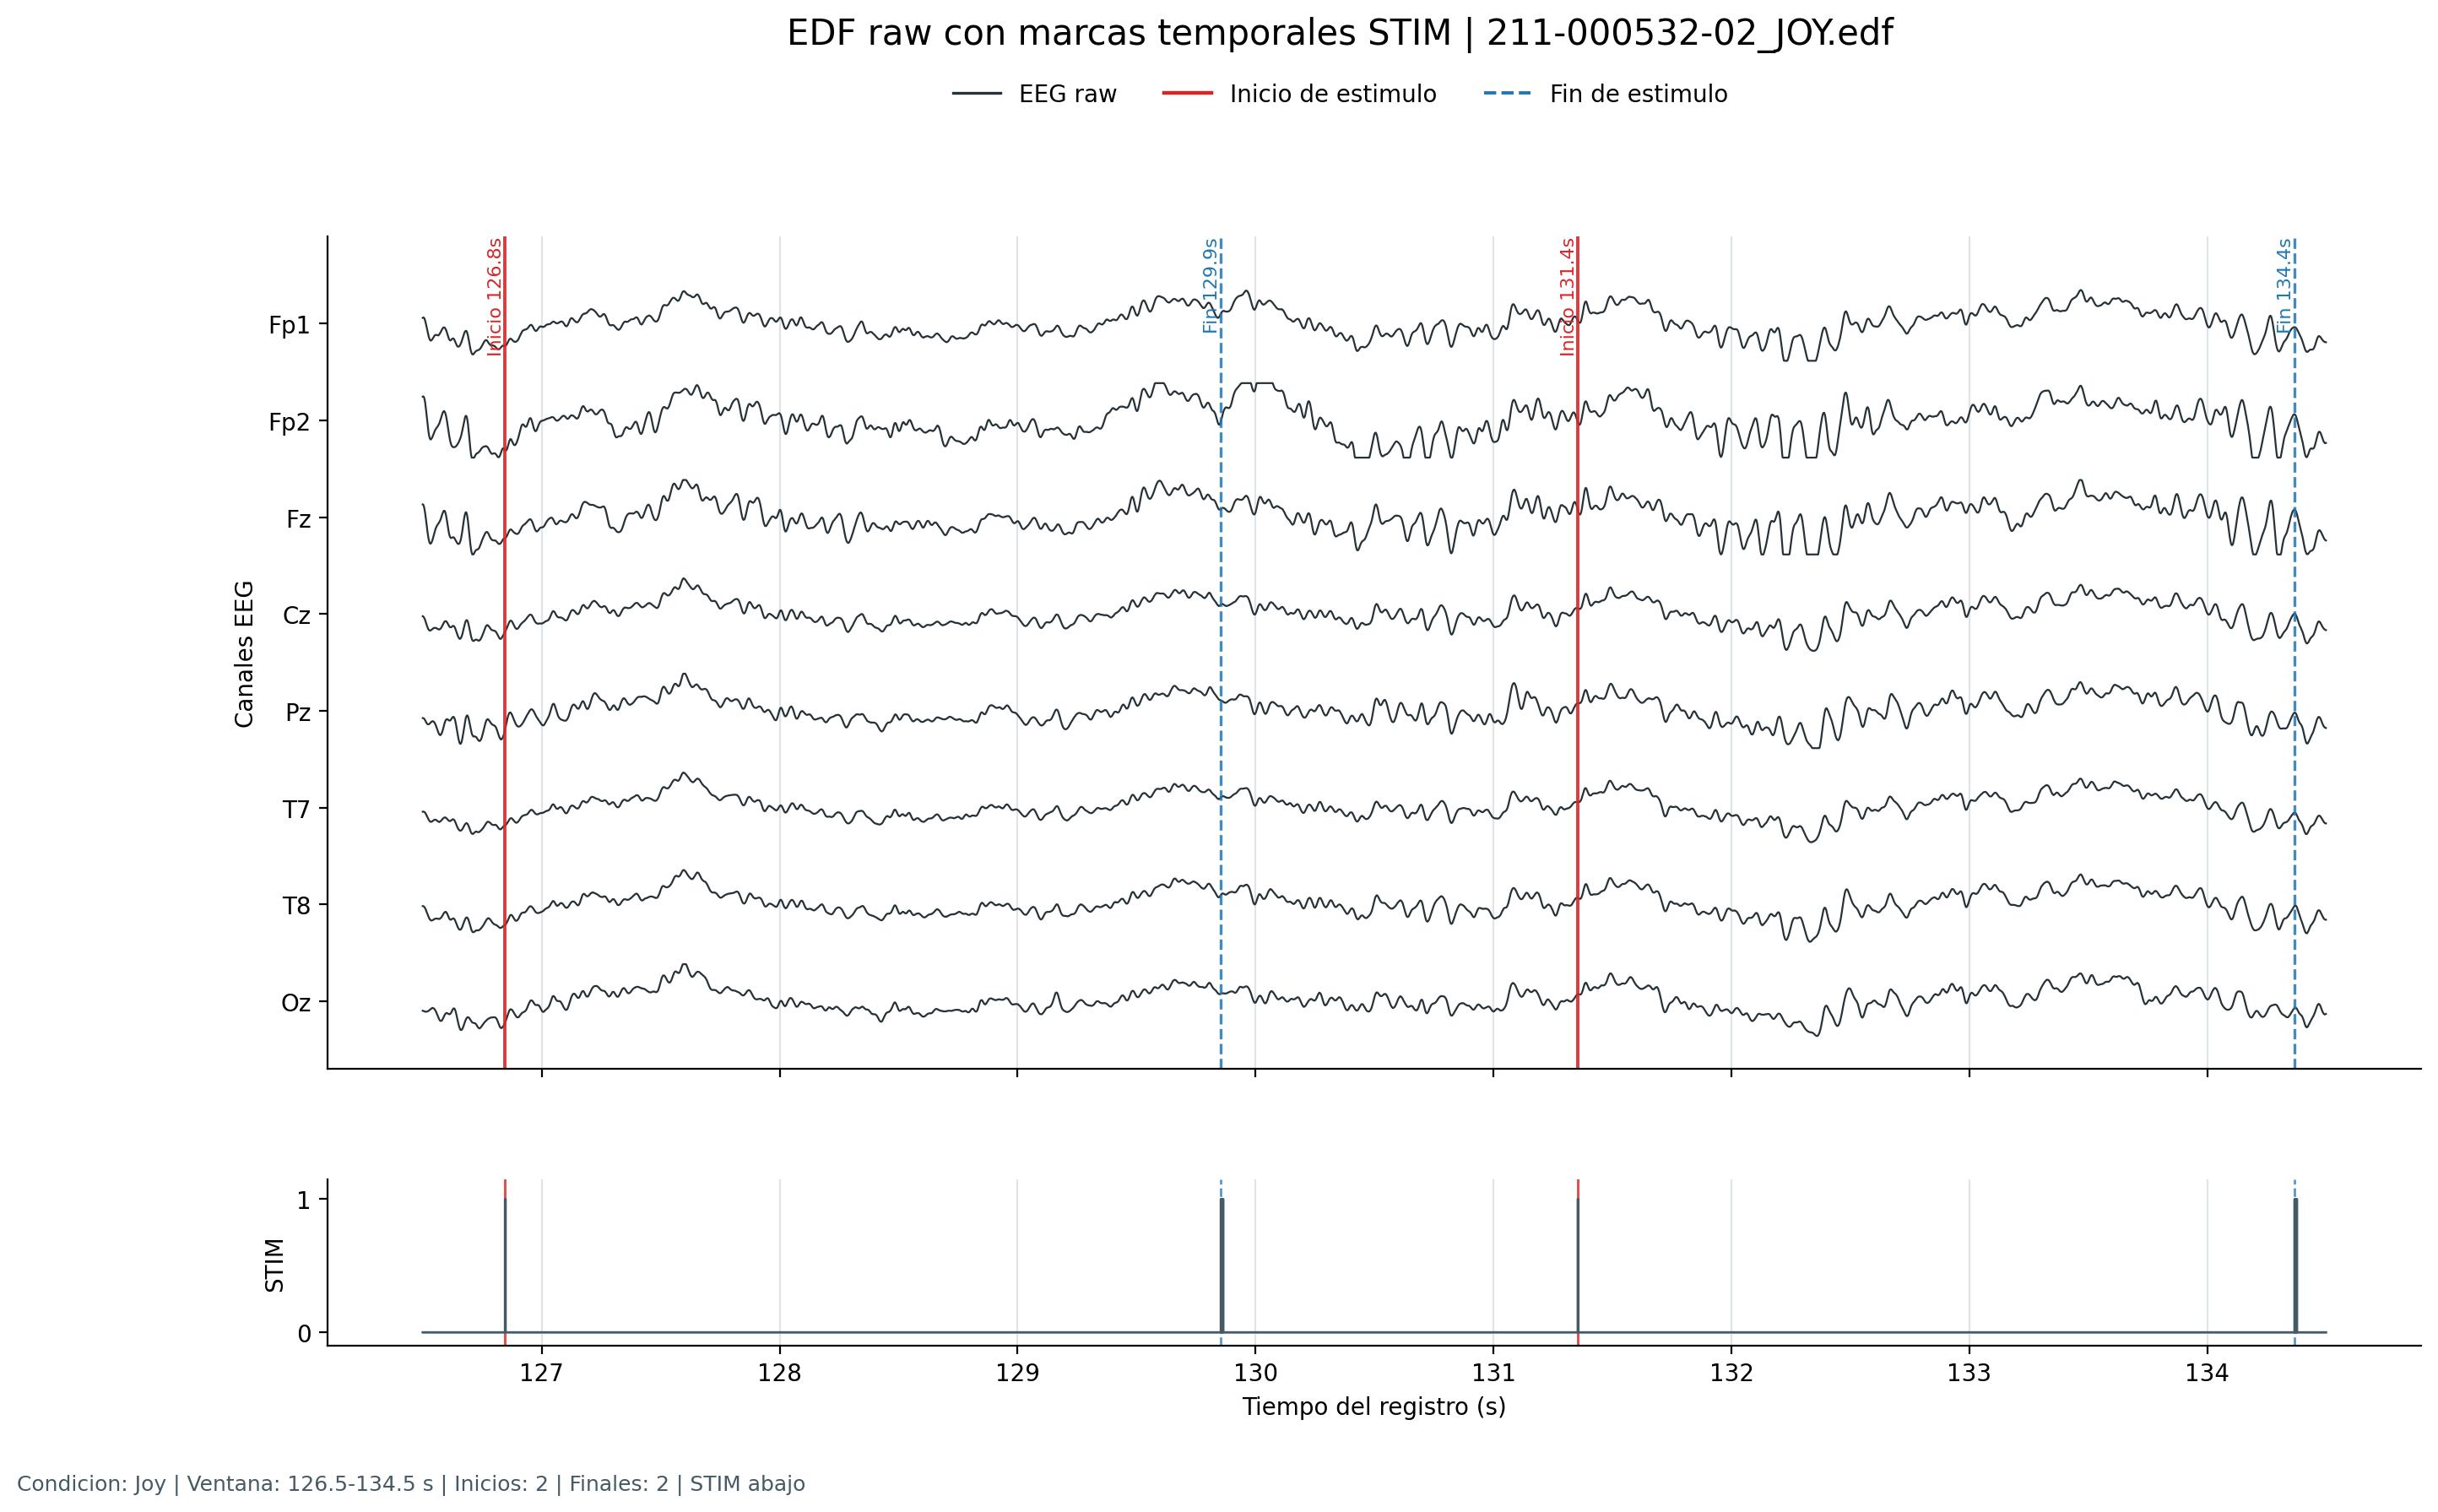
\includegraphics[width=\textwidth]{figs/edf_raw_marcas_temporales.png}
        \end{column}

        \begin{column}{0.49\textwidth}
            \centering
            {\scriptsize\bfseries Épocas preprocesadas consecutivas}\\[-0.5mm]
            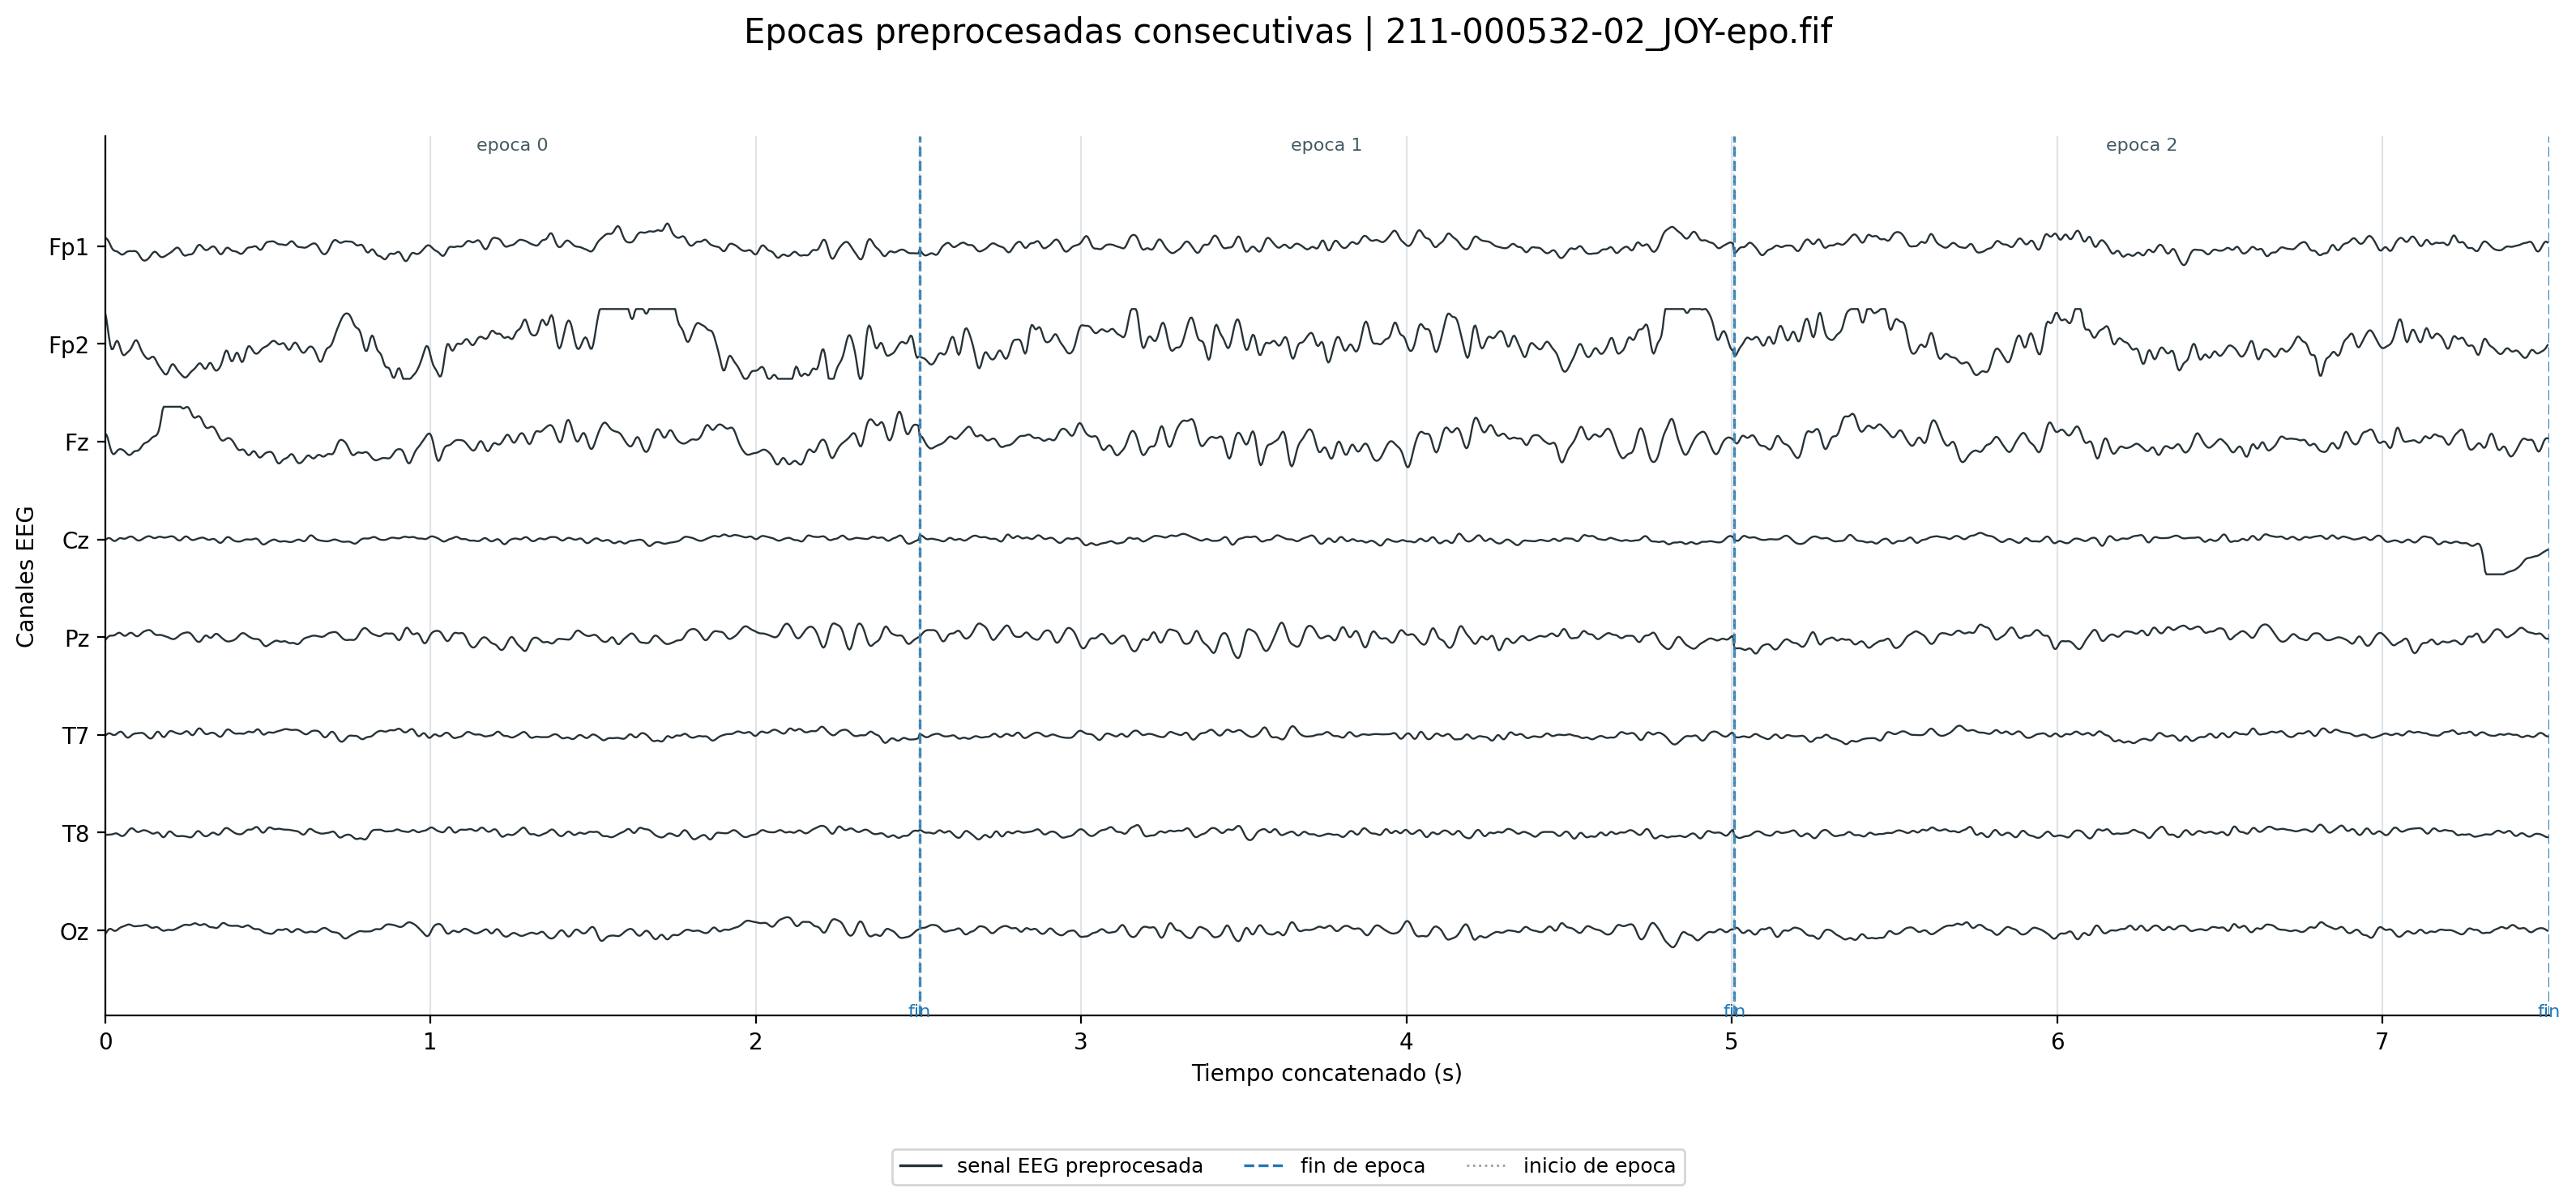
\includegraphics[width=\textwidth]{figs/epocas_consecutivas_marcas.png}
        \end{column}
    \end{columns}
\end{frame}

\begin{frame}{Control de sujetos válidos}
    \centering
    \begin{tikzpicture}[
        card/.style={
            rectangle,
            rounded corners=5pt,
            text width=9.7cm,
            minimum height=1.0cm,
            align=left,
            font=\small,
            inner xsep=10pt,
            draw=black!25
        },
        num/.style={
            circle,
            minimum size=0.58cm,
            font=\bfseries\small,
            text=white,
            fill=urjcred
        }
    ]
        \node[card, fill=blue!10] (a) {
            \hspace{0.55cm}\textbf{Completitud}\\
            \hspace{0.55cm}El sujeto debe tener épocas para JOY, NEUTRO y SAD.
        };
        \node[num, left=0.18cm of a.west] {1};

        \node[card, fill=green!10, below=0.35cm of a] (b) {
            \hspace{0.55cm}\textbf{Balance de épocas}\\
            \hspace{0.55cm}Se revisa que una emoción no quede muy por debajo del resto.
        };
        \node[num, left=0.18cm of b.west] {2};

        \node[card, fill=orange!13, below=0.35cm of b] (c) {
            \hspace{0.55cm}\textbf{Revisión espectral}\\
            \hspace{0.55cm}Se comprueba que la señal conserve una forma espectral compatible con EEG.
        };
        \node[num, left=0.18cm of c.west] {3};

        \node[
            rectangle,
            rounded corners=4pt,
            fill=urjcred!8,
            draw=urjcred!35,
            text width=8.2cm,
            align=center,
            font=\small,
            below=0.45cm of c
        ] {Salida: lista de sujetos aptos para extracción de características.};
    \end{tikzpicture}
\end{frame}

\begin{frame}{Extracción de características}
    \begin{columns}[c,onlytextwidth]
        \begin{column}{0.38\textwidth}
            \centering
            \begin{tikzpicture}[
                bloque/.style={
                    rectangle,
                    rounded corners=4pt,
                    minimum width=4.15cm,
                    minimum height=0.86cm,
                    align=center,
                    font=\small\bfseries,
                    draw=black!45,
                    text width=3.75cm
                },
                detalle/.style={
                    font=\scriptsize,
                    align=center,
                    text width=3.85cm
                },
                flecha/.style={-{Latex[length=2.2mm]}, thick, draw=black!55}
            ]
                \node[bloque, fill=green!14] (epocas) {Épocas limpias};
                \node[detalle, below=0.03cm of epocas] (epocasd)
                    {FIF + sujetos válidos};

                \node[bloque, fill=blue!12, below=0.52cm of epocasd] (psd)
                    {PSD y promedio};
                \node[detalle, below=0.03cm of psd] (psdd)
                    {Welch + media dentro de cada banda};

                \node[bloque, fill=orange!14, below=0.52cm of psdd] (features)
                    {Features finales};
                \node[detalle, below=0.03cm of features]
                    {canal + banda + asimetría};

                \draw[flecha] (epocasd) -- (psd);
                \draw[flecha] (psdd) -- (features);
            \end{tikzpicture}
        \end{column}

        \begin{column}{0.59\textwidth}
            \centering
            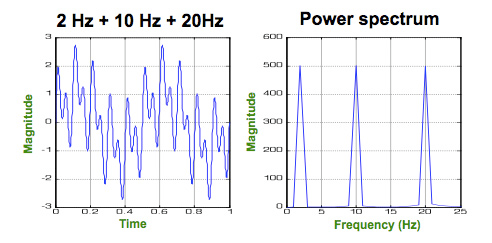
\includegraphics[width=0.82\textwidth]{../memoria/figs/psd.png}

            \vspace{0.20cm}
            \renewcommand{\arraystretch}{1.08}
            {\scriptsize
            \setlength{\tabcolsep}{4pt}
            \begin{tabular}{@{}llc@{}}
                \toprule
                \multicolumn{3}{c}{\textbf{Dataset de entrada al modelo}} \\
                \midrule
                Filas & épocas EEG & 2754 \\
                Columnas & características & 150 \\
                \midrule
                \multicolumn{3}{c}{\textbf{Bloques de características}} \\
                \midrule
                Alpha/Beta & canal + banda, ej. \texttt{FC4\_Beta} & 124 \\
                Asim. Alpha & der.-izq., ej. \texttt{F4-F3} & 26 \\
                \bottomrule
            \end{tabular}
            }

            \vspace{0.18cm}
            {\scriptsize Asimetría: ayuda al modelo a captar diferencias izquierda-derecha.}
        \end{column}
    \end{columns}
\end{frame}

\begin{frame}{Selección de bandas}
    \centering
    \begin{tikzpicture}[
        banda/.style={
            rectangle,
            rounded corners=5pt,
            minimum width=5.25cm,
            minimum height=2.05cm,
            align=center,
            draw=black!35,
            text width=4.75cm,
            inner sep=8pt
        },
        motivo/.style={
            rectangle,
            rounded corners=4pt,
            minimum width=9.8cm,
            minimum height=0.62cm,
            align=center,
            draw=black!25,
            font=\small,
            text width=9.25cm,
            inner sep=5pt
        },
        flecha/.style={-{Latex[length=2.2mm]}, thick, draw=black!55}
    ]
        \node[banda, fill=yellow!20] (alpha) {
            {\Large\bfseries Alpha}\\[1mm]
            {\normalsize 8--12 Hz}\\[2mm]
            {\small estado despierto, tranquilo\\y actividad de referencia}
        };

        \node[banda, fill=green!18, right=0.65cm of alpha] (beta) {
            {\Large\bfseries Beta}\\[1mm]
            {\normalsize 12--30 Hz}\\[2mm]
            {\small atención, procesamiento activo\\y respuesta al estímulo}
        };

        \coordinate (centro) at ($(alpha.south)!0.5!(beta.south)$);

        \node[motivo, fill=urjcred!8, below=0.64cm of centro] (decision) {
            Escucha pasiva: sujeto despierto, ojos cerrados y audio emocional.
        };

        \node[motivo, fill=gray!10, below=0.20cm of decision] {
            Delta, Theta y Gamma quedan fuera del modelo final.
        };

        \coordinate (decisionL) at ([xshift=-2.45cm]decision.north);
        \coordinate (decisionR) at ([xshift=2.45cm]decision.north);
        \draw[flecha] (alpha.south) -- (decisionL);
        \draw[flecha] (beta.south) -- (decisionR);
    \end{tikzpicture}
\end{frame}

\begin{frame}{Entrenamiento y evaluación}
    \centering
    \resizebox{0.98\textwidth}{!}{
    \begin{tikzpicture}[
        carril/.style={
            rounded corners=10pt,
            draw=black!12,
            line width=0.6pt
        },
        etiqueta/.style={
            rectangle,
            rounded corners=6pt,
            minimum width=2.7cm,
            minimum height=0.82cm,
            align=center,
            font=\small\bfseries,
            draw=black!25,
            text width=2.35cm,
            inner sep=5pt
        },
        pasoent/.style={
            rectangle,
            rounded corners=6pt,
            minimum width=2.55cm,
            minimum height=0.78cm,
            align=center,
            font=\scriptsize,
            draw=black!25,
            text width=2.25cm,
            inner sep=5pt
        },
        entrenamiento/.style={
            rectangle,
            rounded corners=8pt,
            minimum width=2.75cm,
            minimum height=1.05cm,
            align=center,
            font=\small,
            draw=black!30,
            fill=yellow!18
        },
        flecha/.style={-{Latex[length=2.2mm]}, thick, draw=black!55}
    ]
        \path[carril, fill=orange!6] (-6.9,0.55) rectangle (1.65,1.85);
        \path[carril, fill=green!6]  (-6.9,-1.35) rectangle (1.65,-0.05);

        \node[etiqueta, fill=orange!18] (general) at (-5.65,1.20) {
            Modelo general
        };

        \node[pasoent, fill=white] (generalcv) at (-2.85,1.20) {
            Stratified\\GroupKFold\\
            por sujeto
        };

        \node[pasoent, fill=white] (generalnorm) at (0.05,1.20) {
            Referencia NEUTRO\\
            sujetos de train
        };

        \node[etiqueta, fill=green!15] (intra) at (-5.65,-0.70) {
            Modelo\\
            por sujeto
        };

        \node[pasoent, fill=white] (intracv) at (-2.85,-0.70) {
            5 \textit{folds}\\temporales
        };

        \node[pasoent, fill=white] (intranorm) at (0.05,-0.70) {
            Referencia NEUTRO\\
            train del sujeto
        };

        \node[entrenamiento] (train) at (3.35,0.25) {
            Entrenamiento\\[-0.6mm]
            {\scriptsize dentro de cada \textit{fold}}
        };

        \node[entrenamiento, fill=urjcred!8] (eval) at (6.45,0.25) {
            Evaluación\\[-0.6mm]
            {\scriptsize métricas y matriz}
        };

        \draw[flecha] (general) -- (generalcv);
        \draw[flecha] (generalcv) -- (generalnorm);
        \draw[flecha] (intra) -- (intracv);
        \draw[flecha] (intracv) -- (intranorm);
        \draw[flecha] (generalnorm.east) -- ++(0.55,0) |- (train.west);
        \draw[flecha] (intranorm.east) -- ++(0.55,0) |- (train.west);
        \draw[flecha] (train) -- (eval);
    \end{tikzpicture}
    }
\end{frame}

\begin{frame}{Explicabilidad}
    \centering
    \resizebox{0.98\textwidth}{!}{
    \begin{tikzpicture}[
        paso/.style={
            rectangle,
            rounded corners=7pt,
            minimum width=2.55cm,
            minimum height=1.05cm,
            align=center,
            font=\small,
            draw=black!30,
            text width=2.25cm,
            inner sep=6pt
        },
        nota/.style={
            rectangle,
            rounded corners=7pt,
            minimum width=8.2cm,
            minimum height=0.65cm,
            align=center,
            font=\scriptsize,
            draw=black!20,
            fill=orange!8
        },
        flecha/.style={-{Latex[length=2mm]}, thick, draw=black!55}
    ]
        \node[paso, fill=green!12] (sujeto) at (-5.3,0.55) {
            Modelo\\por sujeto
        };

        \node[paso, fill=green!8] (folds) at (-2.6,0.55) {
            5 \textit{folds}\\
        };

        \node[paso, fill=yellow!14] (logreg) at (0.1,0.55) {
            Regresión\\logística
        };

        \node[paso, fill=orange!14] (shap) at (2.8,0.55) {
            SHAP\\sobre test
        };

        \node[paso, fill=orange!20] (topomaps) at (5.5,0.55) {
            Topomaps\\de importancia
        };

        \node[nota] at (0.1,-1.15) {
            SHAP no muestra la señal EEG directa: muestra qué canales y bandas influyen más en la decisión del modelo.
        };

        \draw[flecha] (sujeto) -- (folds);
        \draw[flecha] (folds) -- (logreg);
        \draw[flecha] (logreg) -- (shap);
        \draw[flecha] (shap) -- (topomaps);
    \end{tikzpicture}
    }
\end{frame}

\section{Resultados}

\begin{frame}[plain]
    \begin{tikzpicture}[remember picture,overlay]
        \node[align=center, text=black, font=\huge\bfseries, text width=13cm]
            at (current page.center)
            {¿La variabilidad entre sujetos\\[2mm]
            oculta la separación emocional?};
    \end{tikzpicture}
\end{frame}

\begin{frame}{Separabilidad global: PCA}
    \begin{columns}[T,onlytextwidth]
        \begin{column}{0.49\textwidth}
            \centering
            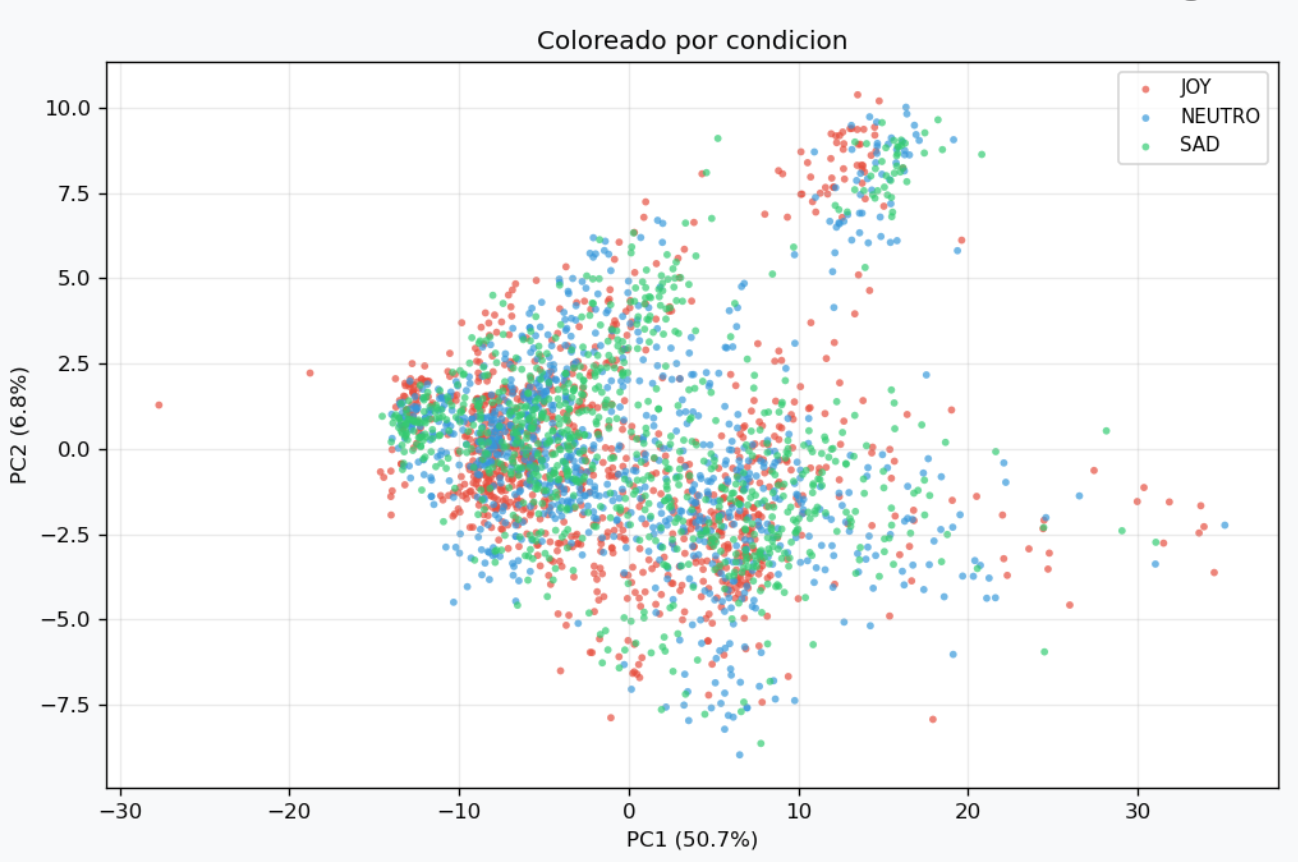
\includegraphics[width=0.94\linewidth]{../memoria/figs/separability/PCA_global_condicion.png}
            \vspace{1mm}

            {\scriptsize Color por condición emocional}
        \end{column}
        \begin{column}{0.49\textwidth}
            \centering
            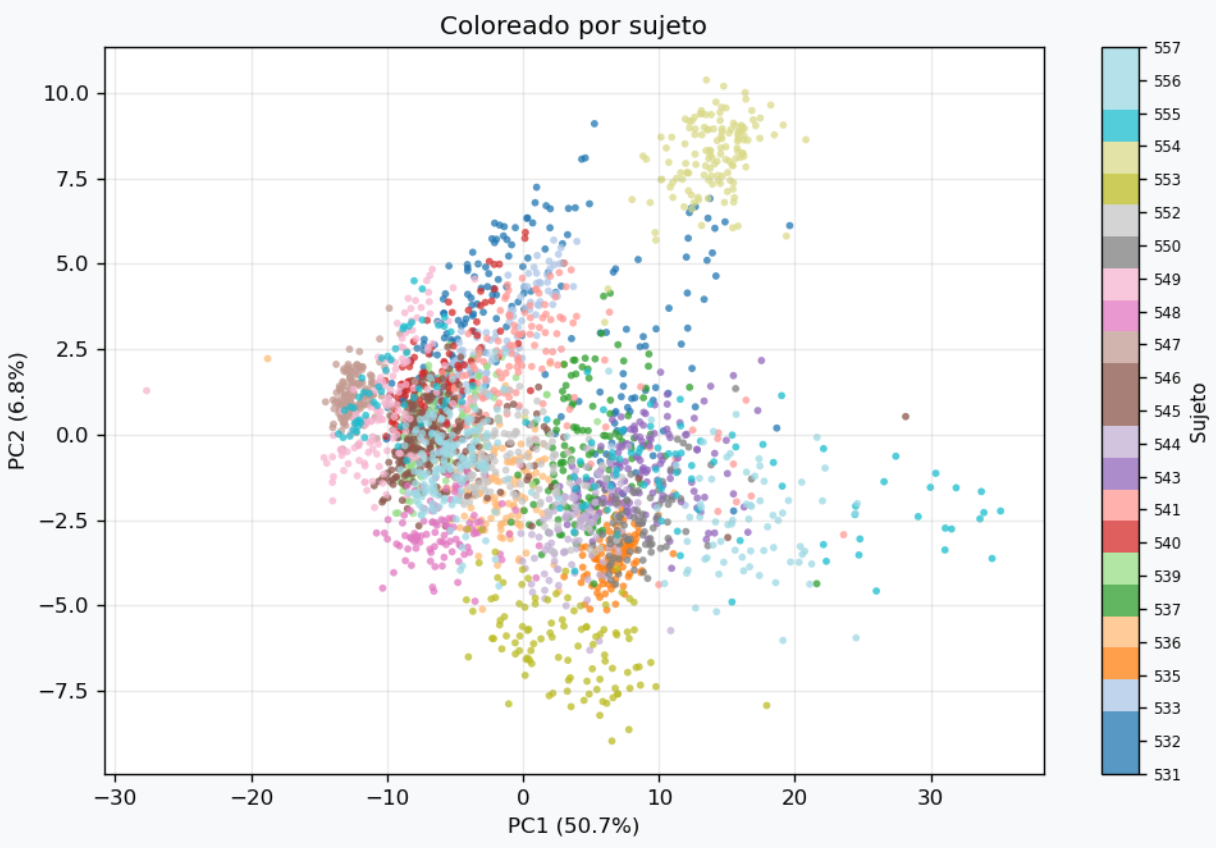
\includegraphics[width=0.94\linewidth]{../memoria/figs/separability/PCA_global_sujeto.png}
            \vspace{1mm}

            {\scriptsize Color por sujeto}
        \end{column}
    \end{columns}

    \vspace{3mm}
    \centering
    {\small La PCA global permite comprobar si la variabilidad principal se organiza mejor por emoción o por diferencias entre participantes.}
\end{frame}

\begin{frame}{Separabilidad global: LDA}
    \begin{columns}[T,onlytextwidth]
        \begin{column}{0.49\textwidth}
            \centering
            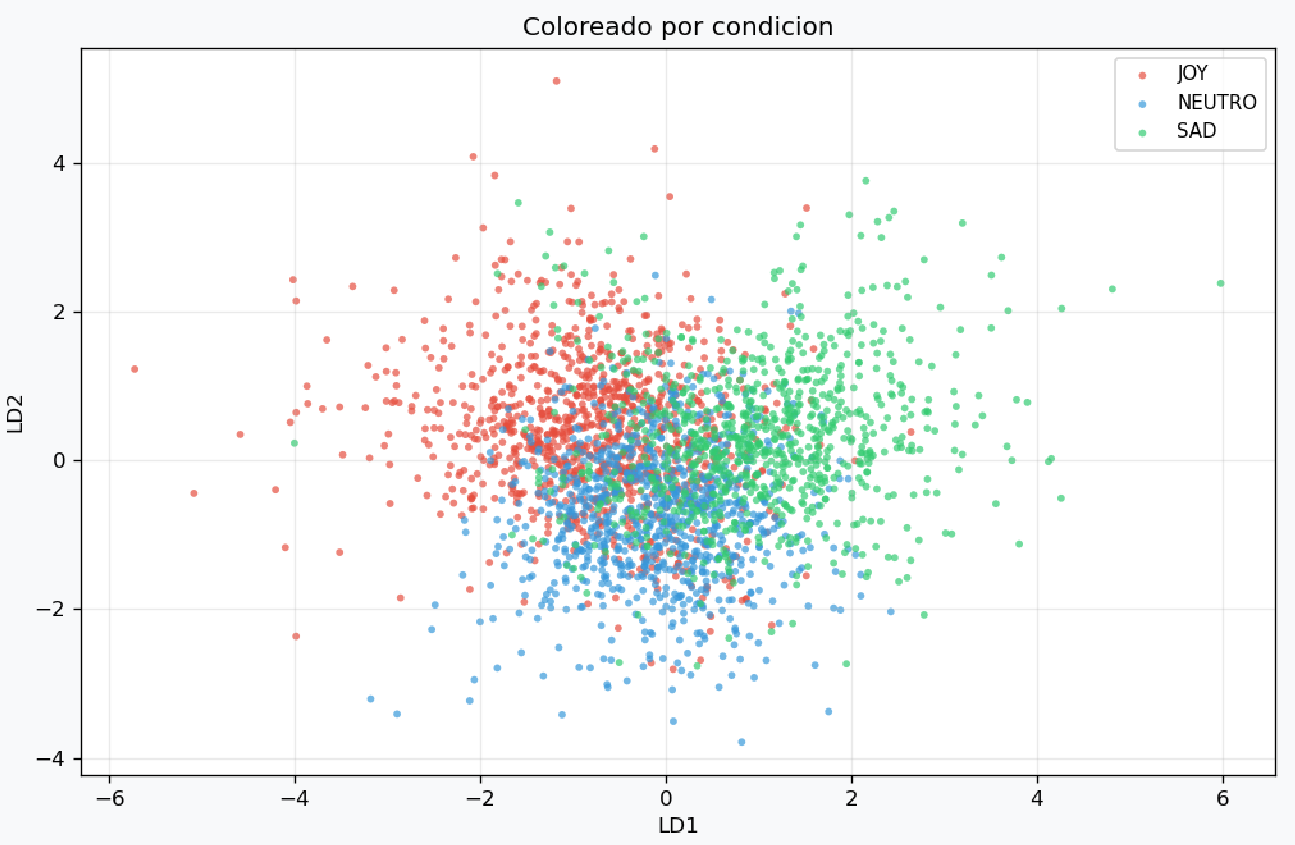
\includegraphics[width=0.94\linewidth]{../memoria/figs/separability/LDA_global_condicion.png}
            \vspace{1mm}

            {\scriptsize Color por condición emocional}
        \end{column}
        \begin{column}{0.49\textwidth}
            \centering
            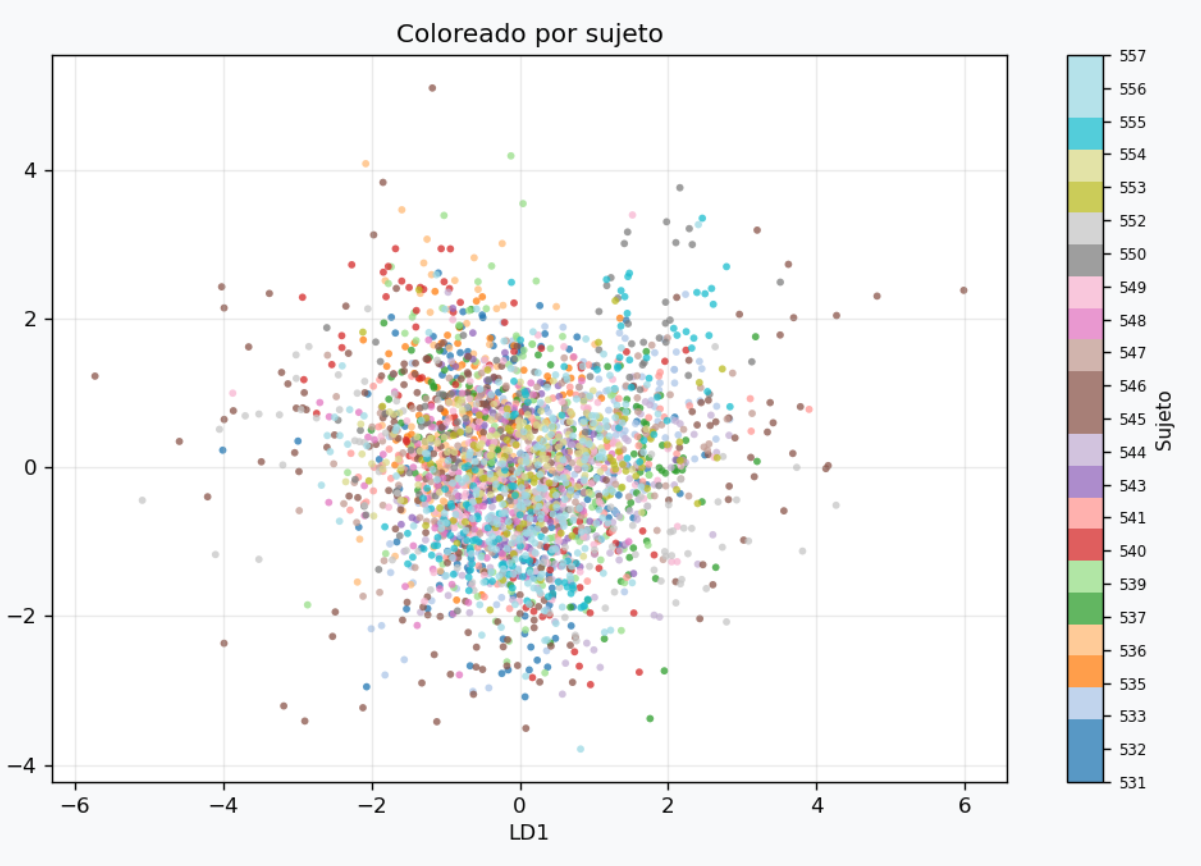
\includegraphics[width=0.94\linewidth]{../memoria/figs/separability/LDA_global_sujeto.png}
            \vspace{1mm}

            {\scriptsize Color por sujeto}
        \end{column}
    \end{columns}

    \vspace{3mm}
    \centering
    {\small La LDA busca una proyección más favorable para separar las emociones, pero sigue mostrando el efecto de la variabilidad entre sujetos.}
\end{frame}

\begin{frame}{Separabilidad por sujeto: PCA}
    \begin{columns}[T,onlytextwidth]
        \begin{column}{0.49\textwidth}
            \centering
            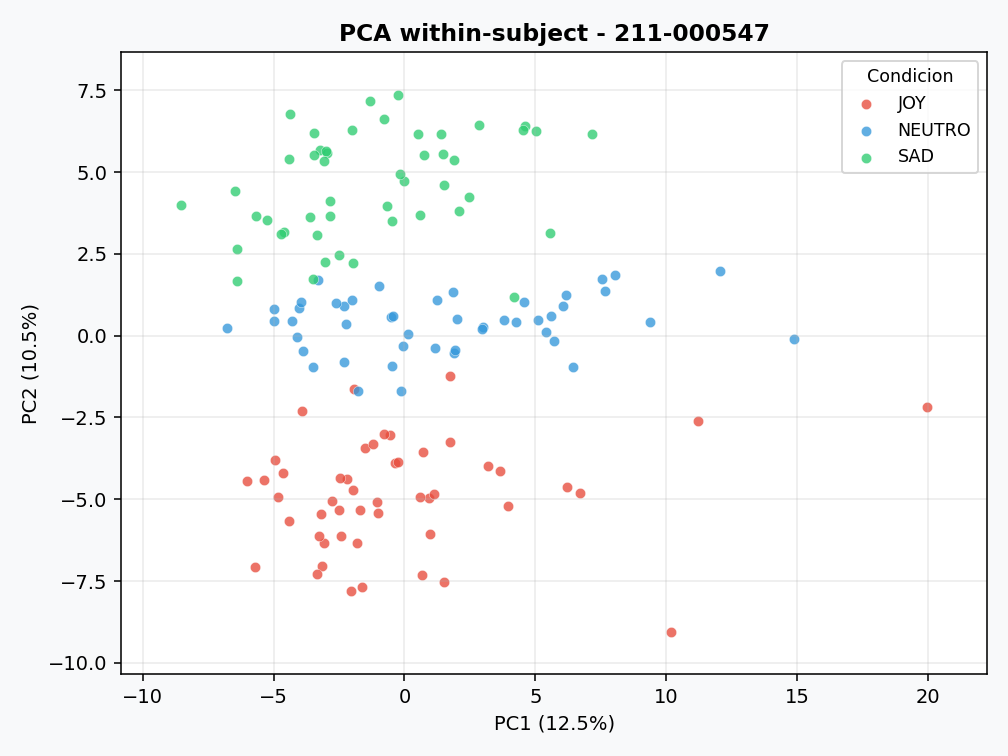
\includegraphics[width=0.88\linewidth]{../memoria/figs/separability/pca_547.png}
            \vspace{1mm}

            {\scriptsize Sujeto 211-000547}
        \end{column}
        \begin{column}{0.49\textwidth}
            \centering
            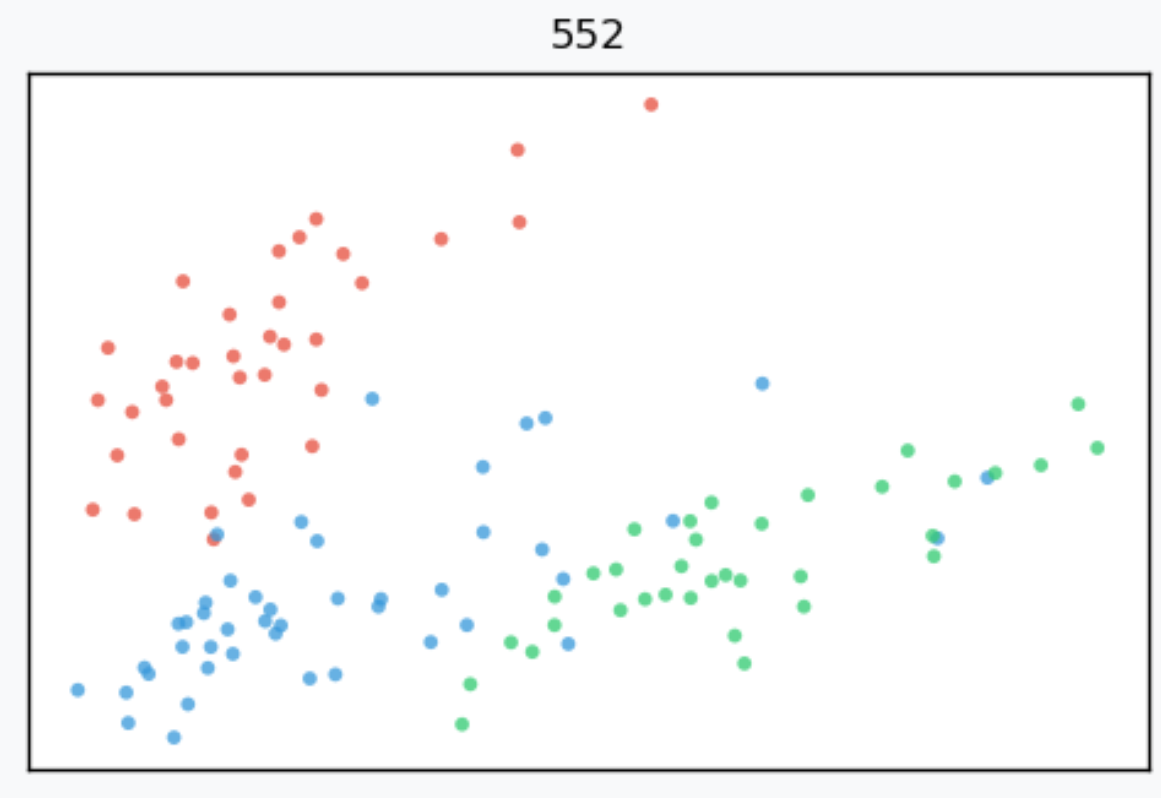
\includegraphics[width=0.88\linewidth]{../memoria/figs/separability/pca_552.png}
            \vspace{1mm}

            {\scriptsize Sujeto 211-000552}
        \end{column}
    \end{columns}

    \vspace{3mm}
    \centering
    {\small Al analizar cada participante por separado, la estructura emocional aparece menos mezclada que en el espacio global.}
\end{frame}

\begin{frame}{Separabilidad por sujeto: LDA}
    \begin{columns}[T,onlytextwidth]
        \begin{column}{0.49\textwidth}
            \centering
            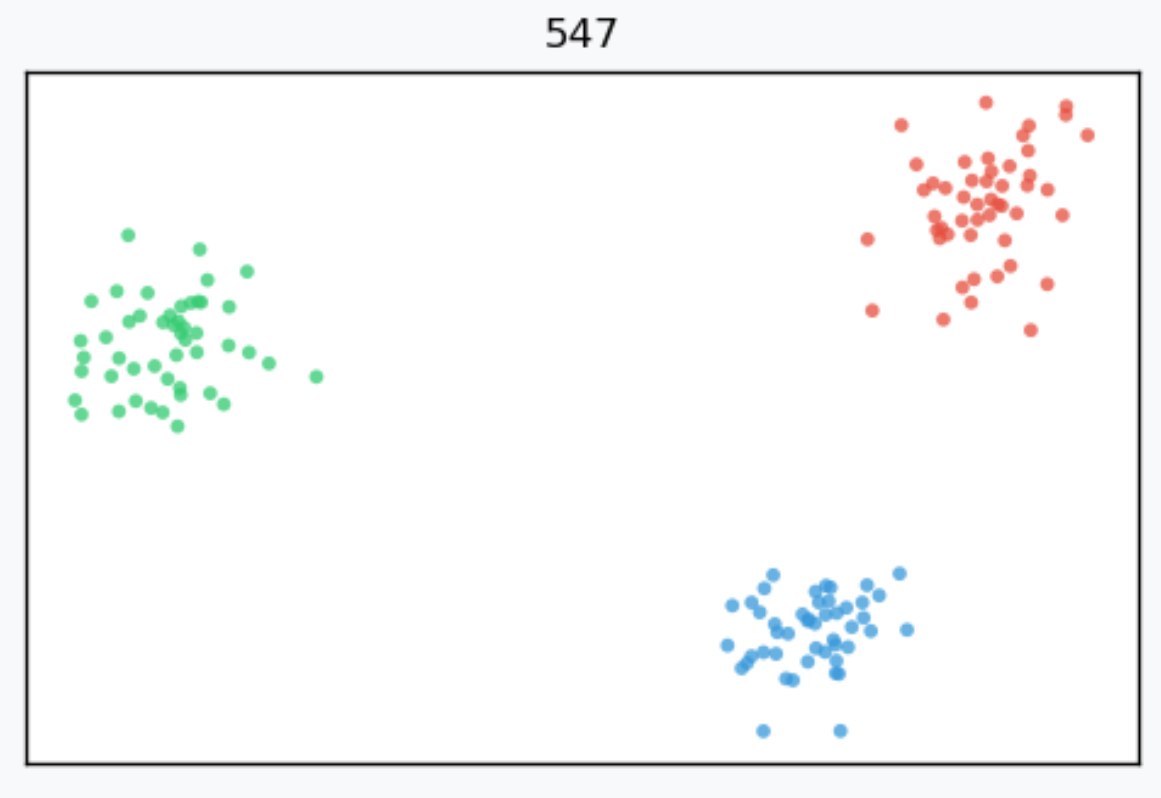
\includegraphics[width=0.88\linewidth]{../memoria/figs/separability/lda_547.png}
            \vspace{1mm}

            {\scriptsize Sujeto 211-000547}
        \end{column}
        \begin{column}{0.49\textwidth}
            \centering
            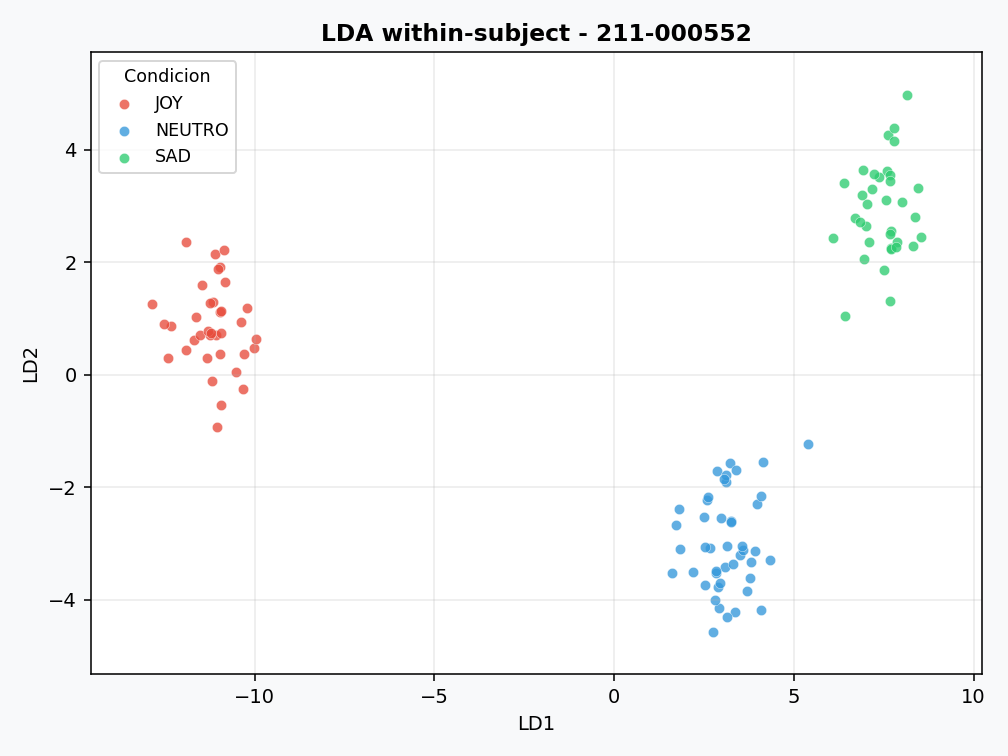
\includegraphics[width=0.88\linewidth]{../memoria/figs/separability/lda_552.png}
            \vspace{1mm}

            {\scriptsize Sujeto 211-000552}
        \end{column}
    \end{columns}

    \vspace{3mm}
    \centering
    {\small La separación dentro de cada sujeto es más clara, lo que anticipa un mejor comportamiento de los modelos personalizados.}
\end{frame}

\begin{frame}{Entrenamiento: regresión logística}
    \begin{columns}[T,onlytextwidth]
        \begin{column}{0.49\textwidth}
            \centering
            {\small\bfseries Modelo general}

            \vspace{1mm}
            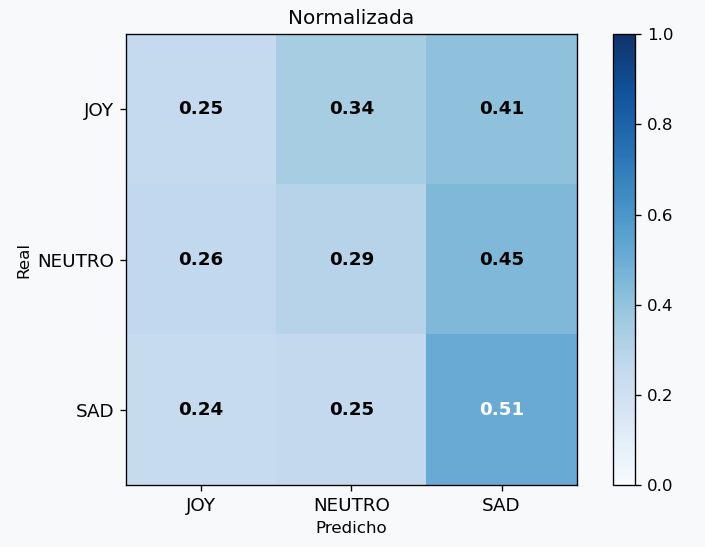
\includegraphics[width=0.92\linewidth]{../memoria/figs/training/all_subjects/log_reg.png}
        \end{column}
        \begin{column}{0.49\textwidth}
            \centering
            {\small\bfseries Modelo por sujeto}

            \vspace{1mm}
            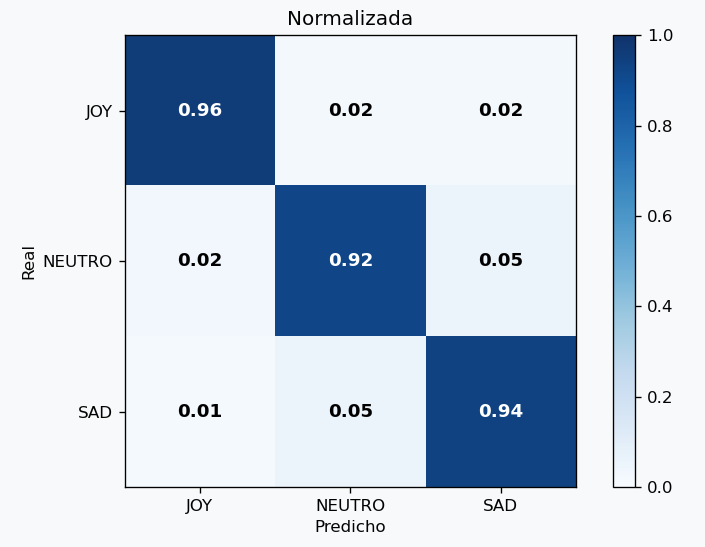
\includegraphics[width=0.92\linewidth]{../memoria/figs/training/within/logreg.png}
        \end{column}
    \end{columns}
\end{frame}

\begin{frame}{Explicabilidad: patrones emocionales}
    \begin{columns}[T,onlytextwidth]
        \begin{column}{0.31\textwidth}
            \begin{beamercolorbox}[rounded=true,sep=0.15cm,wd=\textwidth,center]{block body}
                {\bfseries JOY}\\[1.5mm]
                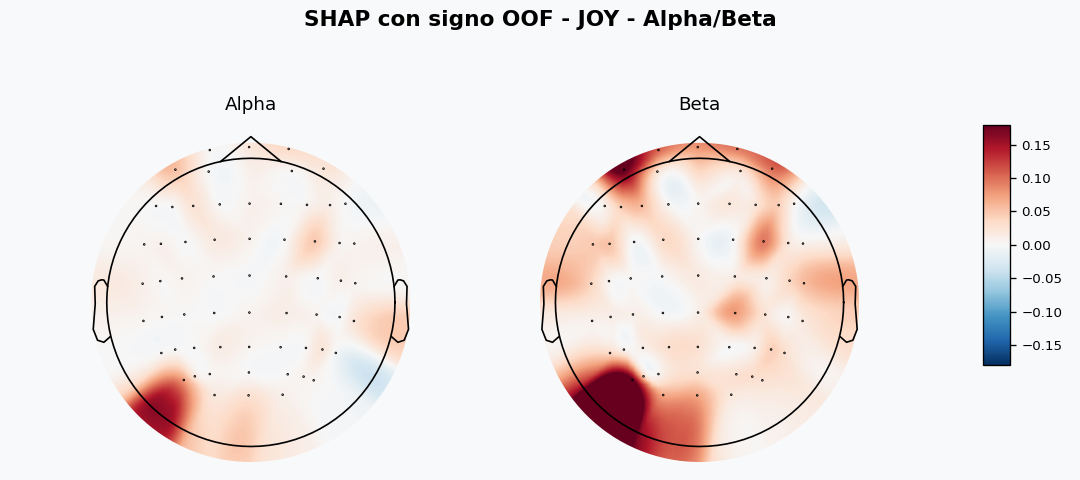
\includegraphics[width=0.90\textwidth]{../memoria/figs/explicabilidad/04_topomap_signed_JOY.png}

                \vspace{0.05cm}
                {\scriptsize frontal y posterior\\mayor implicación}
            \end{beamercolorbox}
        \end{column}

        \begin{column}{0.31\textwidth}
            \begin{beamercolorbox}[rounded=true,sep=0.15cm,wd=\textwidth,center]{block body}
                {\bfseries NEUTRO}\\[1.5mm]
                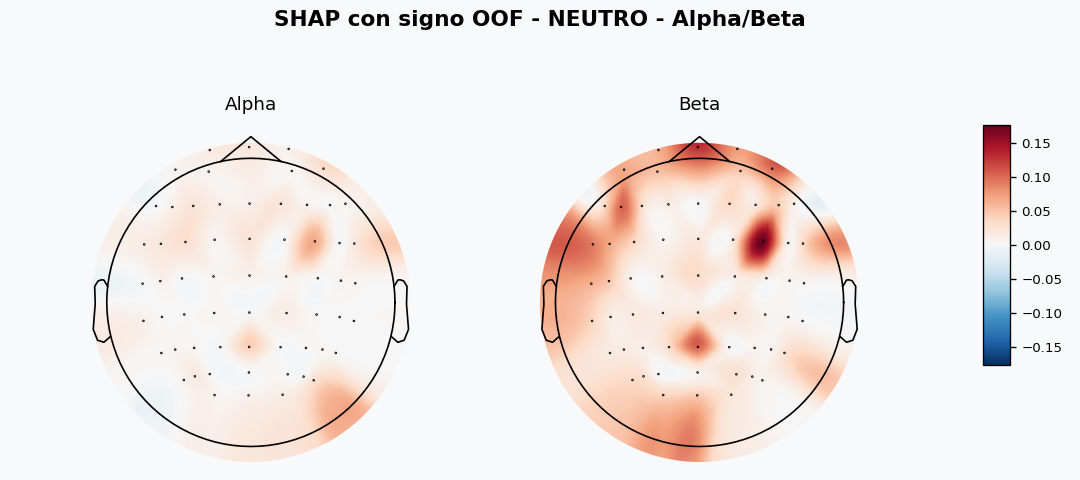
\includegraphics[width=0.90\textwidth]{../memoria/figs/explicabilidad/04_topomap_signed_NEUTRO.png}

                \vspace{0.05cm}
                {\scriptsize distribución más localizada\\referencia emocional}
            \end{beamercolorbox}
        \end{column}

        \begin{column}{0.31\textwidth}
            \begin{beamercolorbox}[rounded=true,sep=0.15cm,wd=\textwidth,center]{block body}
                {\bfseries SAD}\\[1.5mm]
                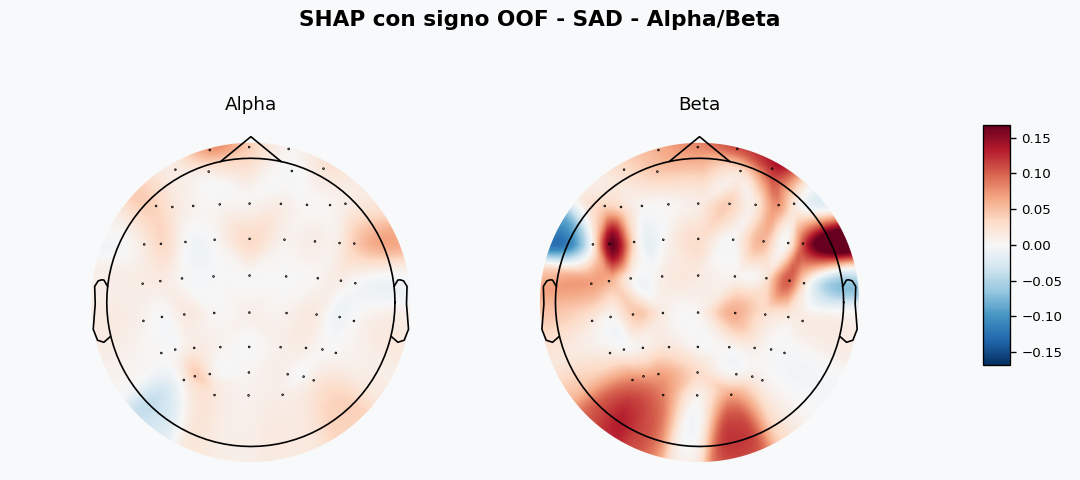
\includegraphics[width=0.90\textwidth]{../memoria/figs/explicabilidad/04_topomap_signed_SAD.png}

                \vspace{0.05cm}
                {\scriptsize temporal y posterior\\frontal menos homogéneo}
            \end{beamercolorbox}
        \end{column}
    \end{columns}

    \vspace{0.25cm}
    \begin{center}
        {\scriptsize Topomaps de importancia: muestran qué zonas y bandas usa el modelo para diferenciar clases.}
    \end{center}
\end{frame}

\section{Conclusiones}

\begin{frame}{Conclusiones y líneas futuras}
    \begin{columns}[T,onlytextwidth]
        \begin{column}{0.49\textwidth}
            \begin{tikzpicture}[
                caja/.style={
                    rectangle,
                    rounded corners=6pt,
                    fill=urjcred!7,
                    draw=urjcred!30,
                    text width=5.35cm,
                    minimum height=0.86cm,
                    align=left,
                    font=\small,
                    inner xsep=8pt
                }
            ]
                \node[font=\large\bfseries, text=urjcred, anchor=west] at (0,0) {Conclusiones};
                \node[caja, anchor=north west] (a) at (0,-0.42) {Sistema completo: dato crudo, preprocesado, entrenamiento y explicabilidad.};
                \node[caja, anchor=north west] (b) at (0,-1.42) {El modelo por sujeto supera al modelo general.};
                \node[caja, anchor=north west] (c) at (0,-2.42) {La variabilidad entre participantes condiciona el análisis de EEG emocional.};
            \end{tikzpicture}
        \end{column}

        \begin{column}{0.49\textwidth}
            \begin{tikzpicture}[
                caja/.style={
                    rectangle,
                    rounded corners=6pt,
                    fill=softblue!8,
                    draw=softblue!35,
                    text width=5.35cm,
                    minimum height=0.86cm,
                    align=left,
                    font=\small,
                    inner xsep=8pt
                }
            ]
                \node[font=\large\bfseries, text=softblue, anchor=west] at (0,0) {Líneas futuras};
                \node[caja, anchor=north west] (a) at (0,-0.42) {Probar con más participantes y emociones para validar el sistema.};
                \node[caja, anchor=north west] (b) at (0,-1.42) {Estudiar transferencia entre sujetos.};
                \node[caja, anchor=north west] (c) at (0,-2.42) {Calibración rápida para acercarlo a contextos clínicos.};
            \end{tikzpicture}
        \end{column}
    \end{columns}
\end{frame}


\end{document}
